%%%%%%%%%%%%%%%%%%%%%%%%%%%%%%%%%%%%%%%%%
% Friggeri Resume/CV
% XeLaTeX Template
% Version 1.1 (9/2/15)
%
% This template has been downloaded from:
% http://www.LaTeXTemplates.com
%
% Original author:
% Adrien Friggeri (adrien@friggeri.net)
% https://github.com/afriggeri/CV
%
% License:
% CC BY-NC-SA 3.0 (http://creativecommons.org/licenses/by-nc-sa/3.0/)
%
% Important notes:
% This template needs to be compiled with XeLaTeX and the bibliography, if used,
% needs to be compiled with biber rather than bibtex.
%
%%%%%%%%%%%%%%%%%%%%%%%%%%%%%%%%%%%%%%%%%

\documentclass[]{friggeri-cv} % Add 'print' as an option into the square bracket to remove colors from this template for printing
%
\addbibresource{bibliography.bib} % Specify the bibliography file to include publications
%
\usepackage{afterpage}
\usepackage{array}
\usepackage{graphicx}
%
%http://tex.stackexchange.com/questions/121891/friggeri-resume-very-different-rendering-in-different-readers
%https://gist.github.com/sway/3101743
%https://coderwall.com/p/r67dyq/using-font-awesome-with-xe-latex
%
\usepackage{fontawesome}
\usepackage{enumitem} % control left margin of itemize environment
%
\newfontfamily{\FA}{FontAwesome}
%
\def\github{\color{gray}{\FA \faGithubSign}}
\def\facebook{\color{gray}{\FA \faFacebookSign}}
\def\linkedin{\color{gray}{\FA \faLinkedinSign}}
\def\phonea{\color{gray}{\FA \faPhone}}
\def\phoneb{\color{gray}{\FA \faPhoneSign}}
\def\phonec{\color{gray}{\FA \faMobile}}
\def\home{\color{gray}{\FA \faHome}}
\def\mail{\color{gray}{\FA \faEnvelopeAlt}}
\def\globe{\color{gray}{\FA \faGlobe}}
%
\def\circleFull{\small\color{gray}{\FA \faCircleFull}\hspace{0.15cm}}
\def\circleEmpty{\small\color{gray}{\FA \faCircleEmpty}\hspace{0.15cm}}
%
\begin{document}
%
\header{Jean-Sébastien}{Gosselin}{Ingénieur Junior \& Doctorant en Hydrogéologie} % Your name and current job title/field •
%
%----------------------------------------------------------------------------------------
%	SIDEBAR SECTION
%----------------------------------------------------------------------------------------
%
\begin{aside} % In the aside, each new line forces a line break
\section{contact}\vspace{5pt}
\home\space 6100 Paul-Gury, \#307
\hspace{0.43cm}Québec, Qc, Canada
\hspace{0.43cm}G1P 4R3\vspace{5pt}
\phoneb\space (581) 996 4070
\href{mailto:jnsebgosselin@gmail.com}{\mail\space jnsebgosselin@gmail.com}
\vspace{10pt}\section{à propos}\vspace{5pt}
32 ans
Canadien
Marié, 1 enfant\vspace{5pt}
\href{http://www.liamg.ca/qui-sommes-nous/jean-sebastien-gosselin/}{\globe\hspace{0.1cm} http://www.liamg.ca}
\href{https://www.linkedin.com/in/jnsebgosselin}{\linkedin\hspace{0.1cm} LinkedIn: jnsebgosselin}
\href{https://www.facebook.com/jnsebgosselin}{\facebook\hspace{0.1cm} Facebook: jnsebgosselin}
\href{https://github.com/jnsebgosselin}{\github\hspace{0.1cm} GitHub: jnsebgosselin}
%
\vspace{10pt}\section{langues}\vspace{5pt}
Français (maternel)
Anglais (courant)
%
\vspace{10pt}\section{intérêts professionnels}\vspace{10pt}
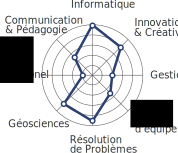
\includegraphics[width=4.5cm]{prof_interests_graph}
%
\vspace{5pt}\section{programmation}\vspace{-5pt}
{\setlength{\extrarowheight}{2pt}%
\begin{tabular}{@{}m{2cm}m{2.5cm}@{}}
  Python 2.7&\hfill\circleFull\circleFull\circleFull\circleFull\circleEmpty
  Matlab&\hfill\circleFull\circleFull\circleFull\circleEmpty\circleEmpty
  LabView&\hfill\circleFull\circleFull\circleEmpty\circleEmpty\circleEmpty
  \LaTeX&\hfill\circleFull\circleFull\circleFull\circleEmpty\circleEmpty
  HTML&\hfill\circleFull\circleEmpty\circleEmpty\circleEmpty\circleEmpty  
  Fortran 95&\hfill\circleFull\circleEmpty\circleEmpty\circleEmpty\circleEmpty  
\end{tabular}}
%
\end{aside}
%{\color{red} $\varheartsuit$}
%
%----------------------------------------------------------------------------------------
%	SUMMARY SECTION
%----------------------------------------------------------------------------------------
%
\section{résumé}
\normalfont{Je suis un professionnel qui termine actuellement un doctorat en hydrogéologie. Je possède une expérience académique et professionnelle diversifiée en physique, en modélisation et en informatique que je souhaite mettre à profit pour résoudre des problèmes techniques concrets et pointus dans le domaine des sciences de la Terre au Québec.}
%
%\setlength{\parindent}{15pt}Je suis une personne sociale en petit groupe qui aime travailler de manière autonome. J'ai un esprit inventif et débrouillard et j'aime élaborer des solutions originales. J'ai un souci du détail très prononcé. Je n'ai pas peur de relever de nouveaux défis, mais j'aime également avoir une certaine constance et routine dans mon travail.\setlength{\parindent}{0pt}
%
%----------------------------------------------------------------------------------------
%	EDUCATION SECTION
%----------------------------------------------------------------------------------------
%
\section{formation}
%
\begin{entrylist}
%------------------------------------------------
\entryMod
{2010--Prés.}
{PhD {\normalfont Sciences de la Terre}}
{INRS - Centre Eau Terre Environnement}
{Projets de recherche - Hydrogéologie}
{(A) Modélisation numérique inverse du transport de chaleur dans les sols pour estimer la recharge des eaux souterraines. (B) Réalisation d'un logiciel informatique pour le traitement, la visualisation et l'interprétation des données météorologiques et des hydrogrammes de puits.}
%------------------------------------------------
\entryMod
{2007--2009}
{MScA {\normalfont Ingénierie}}
{Université du Québec à Rimouski}
{Projet de recherche - Océanographie Physique}
{Conception et programmation d'un modèle numérique pour étudier l'impact de la rugosité de surface de grande échelle sur les taux de fonte de la glace de mer poreuse.}
%------------------------------------------------
\entryMod
{2002--2006}
{BIng {\normalfont Génie Mécanique}}
{Université de Sherbrooke}
{Projet de fin d'étude - Bioingénierie}
{Conception d'une civière d'évacuation pour les personnes à mobilité réduite.}
%------------------------------------------------
\entryAlt
{2000--2002}
{DEC {\normalfont Sciences de la Nature}}
{Cégep de Matane}
%------------------------------------------------
\end{entrylist}
%
%----------------------------------------------------------------------------------------
%	WORK EXPERIENCE SECTION
%----------------------------------------------------------------------------------------
%
\section{expérience}
%
%------------------------------------------------
\begin{entrylist}
  \entryBul
    {2010--Prés.}
    {Institut National de la Recherche Scientifique}
    {Québec, Qc}
    {Candidat au Doctorat - Hydrogéologie}
    {
     \begin{itemize}[leftmargin=*]
       \setlength\itemsep{0pt}
       \item conception, réalisation, distribution et documentation d'un logiciel informatique.                      
       \item interprétation des hydrogrammes de puits et estimation de la recharge pour:
         \begin{itemize}[leftmargin=0.5cm]
           \item 3 projets de caractérisation hydrogéologique sur des bases militaires canadiennes.
           \item le programme d’acquisition de connaissances sur les eaux souterraines en Montérégie-Est.
         \end{itemize}
       \item conception et rédaction de 2 articles scientifiques (en cours).
       \item participation à 7 congrès scientifiques: 4 affiches \& 3 présentations orales.
       \item planification et réalisation de travaux de terrain: sondes thermiques, lysimètres, capteurs de pression, perméamètre de Guelph, échantillonnage du sol et de l'eau.
     \end{itemize}
     }
\end{entrylist}
%------------------------------------------------
\begin{entrylist}
  \entryBul
    {05-09 2005}
    {VélUS - Groupe de R\&D sur le vélo}
    {Sherbrooke, Qc}
    {Stagiaire - Génie Mécanique}
    {
     \begin{itemize}[leftmargin=*]
       \setlength\itemsep{0pt}
       \item étalonnage et validation de 3 capteurs de force pour l'instrumentation d'un vélo de route.
       \item acquisition, analyse et présentation des données recueillies avec le vélo instrumenté.
     \end{itemize}
     }
\end{entrylist}
%En partenariat avec la compagnie québécoise \emph{Cycles Devinci inc.}, j'ai participé au développement d'une nouvelle technologie pour mesurer la déformation et les contraintes appliquées à un cadre de vélo de route en conditions réelles d'utilisation.
%------------------------------------------------
\begin{entrylist}
  \entryBul
    {09-12 2004}
    {Institut Universitaire de Gériatrie de Sherbrooke}
    {Sherbrooke, Qc}
    {Stagiaire de Recherche - Bioingénierie}
    {
     \begin{itemize}[leftmargin=*]
       \setlength\itemsep{0pt}
       \item responsable de l'acquisition de données cinématique auprès de sujets âgés et diabétiques.
       \item participation à l'élaboration d'un protocole pour une étude sur le rétablissement de l'équilibre.
     \end{itemize}
     }
\end{entrylist}
%------------------------------------------------
\begin{entrylist}
  \entryBul
    {01-05 2004}
    {Institut Universitaire de Gériatrie de Sherbrooke}
    {Sherbrooke, Qc}
    {Stagiaire de Recherche - Bioingénierie}
    {
     \begin{itemize}[leftmargin=*]
       \setlength\itemsep{0pt}       
       \item développement d'outils pour l'évaluation du temps de réaction chez l'être humain:
         \begin{itemize}
           \item conception, programmation et documentation d'un logiciel produit avec LabView.
           \item conception et fabrication d'une plateforme électronique avec signal lumineux.
         \end{itemize}
       \item rédaction d'un protocole expérimental pour la calibration de cellules de charge.
     \end{itemize}
     }
\end{entrylist}
%------------------------------------------------
\begin{entrylist}
  \entryBul
    {05-09 2003}
    {Municipalité du Canton d'Orford}
    {Orford, Qc}
    {Préposé à l'inspection des bâtiments}
    {
     \begin{itemize}[leftmargin=*]
       \setlength\itemsep{0pt}  
       \item inspection des nouvelles propriétés et des installations septiques.
       \item gestion des plaintes et des demandes de permis mineurs déposés par les citoyens.
     \end{itemize}
    }
\end{entrylist}

%----------------------------------------------------------------------------------------
%	SIDEBAR SECTION (Second Page)
%----------------------------------------------------------------------------------------
\begin{aside2}
  \section{logiciels informatiques} %\vspace{-5pt}
    \parbox[t]{4.5cm}{{\footnotesize\emph{Intérêt et capacité d'apprentissage de nouveaux logiciels élevés}}}
    \vspace{10pt}{\addfontfeature{Color=lightgray}Bureautique}\vspace{-8pt}
    \begin{tabular}{@{}m{2cm}m{2.5cm}@{}}
      LibreOffice&\hfill\circleFull\circleFull\circleFull\circleFull\circleEmpty
      MS Office&\hfill\circleFull\circleFull\circleFull\circleEmpty\circleEmpty
      Zotero&\hfill\circleFull\circleFull\circleFull\circleFull\circleEmpty
      Thunderbird&\hfill\circleFull\circleFull\circleFull\circleFull\circleEmpty
    \end{tabular}    
    \vspace{-6pt}{\addfontfeature{Color=lightgray}Design Graphique}\vspace{-6pt}
    \begin{tabular}{@{}m{2cm}m{2.5cm}@{}}
      Inkscape&\hfill\circleFull\circleFull\circleFull\circleEmpty\circleEmpty
      GIMP&\hfill\circleFull\circleFull\circleEmpty\circleEmpty\circleEmpty
      MS Visio&\hfill\circleFull\circleFull\circleFull\circleEmpty\circleEmpty
      Scribus&\hfill\circleFull\circleFull\circleEmpty\circleEmpty\circleEmpty 
    \end{tabular}
    \vspace{-6pt}{\addfontfeature{Color=lightgray}Systèmes d'Exploitation}\vspace{-6pt}
    \begin{tabular}{@{}m{2cm}m{2.5cm}@{}}
      Linux&\hfill\circleFull\circleFull\circleFull\circleFull\circleEmpty
      Windows&\hfill\circleFull\circleFull\circleFull\circleEmpty\circleEmpty
    \end{tabular}    
    \vspace{-6pt}{\addfontfeature{Color=lightgray}Logiciels Spécialisés}\vspace{-6pt}
        \begin{tabular}{@{}m{2.5cm}m{2cm}@{}}
          ArcGIS&\hfill\circleFull\circleFull\circleEmpty\circleEmpty\circleEmpty
          \footnotesize{Visual MODFLOW}&\hfill\circleFull\circleEmpty\circleEmpty\circleEmpty\circleEmpty
          Tecplot&\hfill\circleFull\circleEmpty\circleEmpty\circleEmpty\circleEmpty        
        \end{tabular}
  %------------------------------------------------     
  \vspace{-5pt}\section{intérêts personels}\vspace{10pt}
    Musique, Lecture,
    Logiciels Open Source,
    Nouvelles Technologies,
    Badminton et Vélo
\end{aside2}
%
%----------------------------------------------------------------------------------------
%	CERTIFICATION SECTION
%----------------------------------------------------------------------------------------
%
\section{certifications}
  \begin{entrylist}
    \entryFULL
      {2014--Prés.}
      {Ordre des Ingénieurs du Québec}
      {}
      {Ingénieur Junior - License 5055656}
      {}
%------------------------------------------------
    \entryFULL
      {2003--Prés.}
      {ASP Construction}
      {}
      {Attestation cours santé et sécurité générale sur les chantiers de construction\\License 98720}
      {}
\end{entrylist}

%----------------------------------------------------------------------------------------
%	COMPÉTENCE SECTION
%----------------------------------------------------------------------------------------
%
%\section{formations autres}
%  \begin{entrylist}
%    \entryMod
%      {2014}
%      {Microseismic Imaging of Hydraulic Fracturing: Improved Engineering of Unconventional Shale Reservoirs (7 heures)}
%      {}
%      {Shawn Maxwell, IMaGE: Itasca Microseismic and Geomechanical Evaluation\\2014 Distinguished Instructor Short Course, INRS-ETE, Québec, Qc}
%      {}
%------------------------------------------------
%    \entryMod
%      {2014}
%      {Indroduction to Geothermal (6 heures)}
%      {}
%      {Lena Patsa, University of British Columbia\\Formation Divex, INRS-ETE, Québec, Qc}
%      {}
%\end{entrylist}
%
%----------------------------------------------------------------------------------------
%	COMMUNICATION SKILLS SECTION
%----------------------------------------------------------------------------------------
%\newgeometry{left=1.5cm,top=2cm,right=1.5cm,bottom=2cm,nohead,nofoot}
\section{communications notables}
\textbf{\large écrites}\vspace{10pt}\\
\begin{entrylist}
%------------------------------------------------
\entry
{en prép.}
{User Manual and Technical Documentation for WHAT (Well Hydrograph Analysis Toolbox).}
{}
{Jean-Sébastien Gosselin, Christine Rivard et Richard Martel\\\href{https://github.com/jnsebgosselin/WHAT}{https://github.com/jnsebgosselin/WHAT}}
%------------------------------------------------
\entry
{en prép.}
{Application limits of near-surface temperature time series to assess
groundwater recharge.}
{}
{Jean-Sébastien Gosselin, Christine Rivard, Richard Martel et René Lefebvre}
%------------------------------------------------
\entry
{AOÛ 2010}
{Simulation de la percolation induite à l'intérieur d'une glace de mer de première année sous l'effet du blocage hydrodynamique d'une quille de glace; Analyse de l'impact sur le flux de chaleur latente glace-océan.}
{}
{Jean-Sébastien Gosselin\\\emph{Mémoire de Maîtrise en Ingénierie, Université du Québec à Rimouski, Rimouski, 111 pages.}}
%------------------------------------------------
\end{entrylist}
\textbf{\large orales et par affiches}\vspace{10pt}\\
\begin{entrylist}
%------------------------------------------------
\entry
{MAI 2015}
{A new user-friendly tool to estimate groundwater recharge from daily weather data and well hydrographs.}
{}
{Jean-Sébastien Gosselin, Christine Rivard, Richard Martel et René Lefebvre\\
 \emph{Présentation Orale (Anglais), Joint assembly AGU-GAC-MAC-CGU, Montréal}}
%------------------------------------------------
\entry
{MAI 2014}
{Exploitation des hydrogrammes de puits du projet PACES en Montérégie Est.}
{}
{Jean-Sébastien Gosselin, Marc Laurencelle, Christine Rivard, Richard Martel et René Lefebvre\\\emph{Présentation par Affiche (Français), 82e congrès de l'ACFAS, Université Concordia, Montréal}}
%------------------------------------------------
\entry
{SEP 2013}
{Estimating recharge from observed well hydrographs combined with meteorological data.}
{}
{Jean-Sébastien Gosselin, Christine Rivard, Richard Martel et Claudio Paniconi\\\emph{GéoMontréal 2013, Hilton Montreal Bonaventure Hotel, Montréal}}
%------------------------------------------------
%\entry
%{MAR 2012}
%{Revue de la méthode d'estimation de la recharge à partir de mesures superficielles de températures}
%{Présentation par Affiche - Français}
%{Jean-Sébastien Gosselin, Christine Rivard, Claudio Paniconi et Richard Martel\\JSTE 2012, INRS-ETE, Québec}
%------------------------------------------------
\entry
{SEP 2012}
{Critical evaluation of the use of superficial temperature measurements for recharge assessment.}
{}
{Jean-Sébastien Gosselin, Christine Rivard, Claudio Paniconi et Richard Martel\\\emph{Présentation par Affiche (Anglais), 39th IAH Congress, Falls Hotel, Niagara Falls}}
%------------------------------------------------
\entry
{AOÛ 2011}
{Applicability of temperature profile techniques for estimating recharge fluxes through the vadose zone.}
{}
{Jean-Sébastien Gosselin, Christine Rivard, Claudio Paniconi et Richard Martel\\\emph{Présentation Orale (Anglais), GeoHydro 2011, Palais des Congrès, Québec}}
%------------------------------------------------
%\entry
%{OCT 2010}
%{Développement d'une stratégie d'estimation de la recharge à l'échelle régionale: étude %de cas en Montérégie Est.}
%{Présentation par Affiche - Français}
%{Jean-Sébastien Gosselin, Christine Rivard, Richard Martel et Claudio Paniconi\\Colloque sur les Eaux Souterraines, Université du Québec à Chicoutimi, Chicoutimi}
\end{entrylist}


%----------------------------------------------------------------------------------------

%----------------------------------------------------------------------------------------
%	PUBLICATIONS SECTION
%----------------------------------------------------------------------------------------

%\section{publications}

%\printbibsection{article}{article in peer-reviewed journal} % Print all articles from the bibliography

%\printbibsection{book}{books} % Print all books from the bibliography

%\begin{refsection} % This is a custom heading for those references marked as "inproceedings" but not containing "keyword=france"
%\nocite{*}
%\printbibliography[sorting=chronological, type=inproceedings, title={international peer-reviewed conferences/proceedings}, notkeyword={france}, heading=subbibliography]
%\end{refsection}

%\begin{refsection} % This is a custom heading for those references marked as "inproceedings" and containing "keyword=france"
%\nocite{*}
%\printbibliography[sorting=chronological, type=inproceedings, title={local peer-reviewed conferences/proceedings}, keyword={france}, heading=subbibliography]
%\end{refsection}

%\printbibsection{misc}{other publications} % Print all miscellaneous entries from the bibliography

%\printbibsection{report}{research reports} % Print all research reports from the bibliography

\end{document}
